\documentclass[finnish]{report}
\usepackage[utf8]{inputenc}
\usepackage[T1]{fontenc}
\usepackage{graphicx}
\usepackage{babel}
\usepackage{float}
\restylefloat{figure}

% Luvuille otsikkona pelkkä luvun nimi ja numero
\makeatletter
\def\@makechapterhead#1{%
  \vspace*{50\p@}%
  {\parindent \z@ \raggedright \normalfont
    \interlinepenalty\@M
    \Huge\bfseries  \thechapter.\quad #1\par\nobreak
    \vskip 40\p@
  }}
\makeatother


\begin{document}

\title{Tietokantasovellus - FlexDo}
\author{Henry Carlson}
\maketitle

\tableofcontents

\chapter{Johdanto}
Tavoitteena on kehittää tehokas järjestelmä tehtävien hallintaan. Tehtävät tulisi voida priorisoida, ja lajitella omiin luokkiinsa.

\section{Järjestelmän tarkoitus}
Järjestelmän perusta on priorisoitu tehtävälista. Järjestelmän tulisi sallia käyttäjän lisätä tehtäviä listalle, asettaa tehtäville prioriteetti, ja selata niitä eri järjestyksissä (mm. prioriteetin mukaan). Lisäksi tehtävät tulisi voida luokitella erillisiin kategorioihin, mielellään hierarkisesti.

\section{Toteutus}
Järjestelmä toteutetaan Java/Tomcat verkkosovelluksena, tietokantajärjestelmänä PostgreSQL. Järjestelmän tulisi olla käytettävissä puhtaasti html muotoisena, mutta käyttöä helpottavia lisätoimintoja voidaan tarvittaessa toteuttaa javascriptillä.


\chapter{Yleiskuva järjestelmästä}

\section{Käyttäjäryhmät}
\begin{description}
  \item[Käyttäjä] \hfill \\
    Rekisteröitynyt ja järjestelmään sisäänkirjautunut käyttäjä
\end{description}

\section{Käyttötapaukset}
\begin{description}
  \item[Kirjautuminen]
  \item[Rekisteröityminen]
  \item[Askareen lisäys] \hfill \\
    Käyttäjä voi lisätä uuden askareen. Askareelle annetaan lisätessä nimi, mahdollinen kuvaus ja prioriteetti.
  \item[Askareen muokkaus] \hfill \\
    Käyttäjä voi muokata järjestelmässä olevan askareen prioriteettia, nimeä sekä kuvausta.
  \item[Askareen poisto] \hfill \\
    Käyttäjä voi poistaa askareen järjestelmässä. Poiston yhteydessä voidaan joko merkitä askare suoritetuksi, jolloin se jää järjestelmään erilliseen kategoriaan kirjanpitoa varten, taikka poistaa askare kokonaan järjestelmästä.
  \item[Askareiden selaus prioriteetin mukaan] \hfill \\
    Käyttäjä voi selata järjestelmässä olevia askareita prioriteettijärjestyksessä.
  \item[Luokkien lisäys ja poisto] \hfill \\
    Käyttäjä voi lisätä ja poistaa järjestelmässä olevia askareiden luokkia.
  \item[Askareiden luokittelu] \hfill \\
    Käyttäjä voi liittää askareen luokkaan, taikka poistaa sen luokasta. Yksi askare voi kuulua useaan luokkaan.
  \item[Askareiden selaus luokittain] \hfill \\
    Käyttäjä voi selata järjestelmässä olevia askareita luokan mukaan.
  \item[Suoritettujen askareiden selaus] \hfill \\
    Käyttäjä voi selata suoritettuja askareita suoritusajankohdan mukaan järjestettynä.
  \item[Luokkien hierarkkinen järjestely] \hfill \\
    Käyttäjä voi asettaa luokkia toistensa alaluokiksi, muodostaen hierarkisen luokkarakenteen.
\end{description}


\chapter{Järjestelmän tietosisältö}

\begin{figure}[H]
\centering
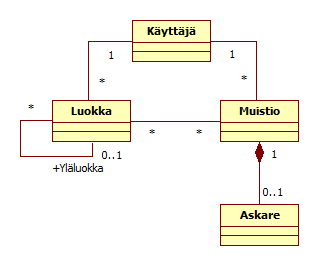
\includegraphics[width=0.5\textwidth]{kasitekaavio}
\caption{Käsitekaavio}
\end{figure}

\section{Tietokohteet}

\paragraph{Tietokohde: Käyttäjä} ~\\

\begin{tabular}{ | l | l | l | }
  \hline
  Attribuutti & Arvojoukko & Kuvailu \\ \hline
  Nimi & Merkkijono & Käyttäjätunnus \\
  Salasana & Merkkijono, pituus tiivistefunktion mukaan & Käyttäjän salasanaa vastaava tiiviste \\
  \hline
\end{tabular}


\paragraph{Tietokohde: Muistio} ~\\

\begin{tabular}{ | l | l | l | }
  \hline
  Attribuutti & Arvojoukko & Kuvailu \\ \hline
  Käyttäjä & Vieras avain & Linkki muistion omistavaan käyttäjään \\
  Nimi & Merkkijono & Muistion nimi \\
  Sisältö & Merkkijono & Muistion sisältö \\
  Luontiaika & Aika ja päivämäärä & Muistion luomisaijankohta \\
  \hline
\end{tabular}

\vspace{5pt}
Muistio koostuu otsikosta ja tekstisisällöstä. Muistiosta voidaan tehdä askare linkkamalla siihen askare-tietkohde.


\paragraph{Tietokohde: Askare} ~\\

\begin{tabular}{ | l | l | l | }
  \hline
  Attribuutti & Arvojoukko & Kuvailu \\ \hline
  Muistio & Vieras avain & Linkki muistioon, josta askareen tietosisältö löytyy \\
  Prioriteetti & Kokonaisluku & Askareen prioriteetti \\
  Sulkemisaika & Aika ja päivämäärä & Askareen sulkemisajankohta, jos askare on suoritettu \\
  \hline
\end{tabular}

\vspace{5pt}
Tietokannan askare-taulu sisältää kaiken tarvittavan metatiedon jolla muistiosta voidaan tehdä askare.
Jokaiseen askareeseen liittyy tasan yksi muistio.


\paragraph{Tietokohde: Luokka} ~\\

\begin{tabular}{ | l | l | l | }
  \hline
  Attribuutti & Arvojoukko & Kuvailu \\ \hline
  Käyttäjä & Vieras avain & Linkki luokan omistavaan käyttäjään \\
  Nimi & Merkkijono & Luokan nimi \\
  Yläluokka & Vieras avain & Linkki mahdolliseen luokan yläluokkaan \\
  \hline
\end{tabular} \\

\vspace{5pt}
Luokat voidaan järjestää hierarkiaan yläluokka-suhteen mukaan. Jokainen muistio voi kuulua yhteen tai useampaan luokkaan.


\chapter{Relaatiotietokantakaavio}

\begin{figure}[H]
\centering
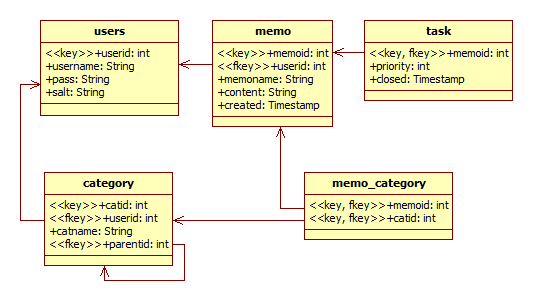
\includegraphics[width=0.75\textwidth]{relaatiotietokantakaavio}
\caption{Relaatiotietokantakaavio}
\end{figure}


\chapter{Järjestelmän yleisrakenne}

% TODO


\chapter{Käyttöliittymä ja järjestelmän komponentit}

% TODO


\chapter{Asennustiedostot}

Asenna sovellus lisäämällä Tomcat:iin sovelluspaketti (.war). Luo sen jälkeen sovellukselle 'FlexDo/META-INF/context.xml'-tiedosto kopioimalla mallitiedosto 'FlexDo/META-INF/context.xml.dist', ja muuttamalla kohdat 'USERNAME', 'PASSWORD' ja 'DBNAME' ympäristön mukaisiksi.


\chapter{Käynnistys-/käyttöohje}

Asennuksen jälkeen sovelluksen tulisi löytyä palvelimelta aliosoitteesta '/FlexDo/index'.
Kirjaudu sisään sovellukseen hallinnointitunnuksilla (oletuksena käyttäjänimi 'admin', salasana 'admin'), ja luo tarvittavat käyttäjätunnukset.
% TODO - Tietokannan populointi


\chapter{Testaus, tunnetut bugit ja puutteet, jatkokehitysideat}

\section{Testaus}

Sovellusta on testattu lähinnä käyttämällä sovellusta normaalisti sovelluksen kehityksen yhteydessä. Mitään varsinaista järjestelmällistä testausta (testaussuunitelma, automatisoidut testitapaukset jne.) ei sovellukselle ole tehty.

\section{Jatkokoehitysideoita}

\begin{itemize}
  \item Askareiden haku
  \item Askareiden aikataulutus
  \item Askareiden välisiä linkkejä (wiki-tyyli)
  \item Askareiden välisiä vaativuuksia (Tehtävä B ei ole suoritettavissa ennenkuin tehtävä A on suoritettu)
  \item Projektinäkymä (kartoitettu näkymä aikataulusta ja askareiden väisistä riippuvuuksista)
\end{itemize}


\chapter{Omat kokemukset}


\end{document}